%%%%%%%%%%%%%%%%%%%%%%%%%%%%%%%%%%%%%%%%%
% Short Sectioned Assignment
% LaTeX Template
% Version 1.0 (5/5/12)
%
% This template has been downloaded from:
% http://www.LaTeXTemplates.com
%
% Original author:
% Frits Wenneker (http://www.howtotex.com)
%
% License:
% CC BY-NC-SA 3.0 (http://creativecommons.org/licenses/by-nc-sa/3.0/)
%
%%%%%%%%%%%%%%%%%%%%%%%%%%%%%%%%%%%%%%%%%

%----------------------------------------------------------------------------------------
%	PACKAGES AND OTHER DOCUMENT CONFIGURATIONS
%----------------------------------------------------------------------------------------

\documentclass[paper=a4, fontsize=11pt]{scrartcl} % A4 paper and 11pt font size

\usepackage[T1]{fontenc} % Use 8-bit encoding that has 256 glyphs
\usepackage{fourier} % Use the Adobe Utopia font for the document - comment this line to return to the LaTeX default
\usepackage[english]{babel} % English language/hyphenation
\usepackage{amsmath,amsfonts,amsthm} % Math packages
\usepackage{csvsimple}
\usepackage{graphicx}

\usepackage{lipsum} % Used for inserting dummy 'Lorem ipsum' text into the template

\usepackage{sectsty} % Allows customizing section commands
\allsectionsfont{\centering \normalfont\scshape} % Make all sections centered, the default font and small caps

\usepackage{fancyhdr} % Custom headers and footers
\pagestyle{fancyplain} % Makes all pages in the document conform to the custom headers and footers
\fancyhead{} % No page header - if you want one, create it in the same way as the footers below
\fancyfoot[L]{} % Empty left footer
\fancyfoot[C]{} % Empty center footer
\fancyfoot[R]{\thepage} % Page numbering for right footer
\renewcommand{\headrulewidth}{0pt} % Remove header underlines
\renewcommand{\footrulewidth}{0pt} % Remove footer underlines
\setlength{\headheight}{13.6pt} % Customize the height of the header

\numberwithin{equation}{section} % Number equations within sections (i.e. 1.1, 1.2, 2.1, 2.2 instead of 1, 2, 3, 4)
\numberwithin{figure}{section} % Number figures within sections (i.e. 1.1, 1.2, 2.1, 2.2 instead of 1, 2, 3, 4)
\numberwithin{table}{section} % Number tables within sections (i.e. 1.1, 1.2, 2.1, 2.2 instead of 1, 2, 3, 4)

\setlength\parindent{0pt} % Removes all indentation from paragraphs - comment this line for an assignment with lots of text

%----------------------------------------------------------------------------------------
%	TITLE SECTION
%----------------------------------------------------------------------------------------

\newcommand{\horrule}[1]{\rule{\linewidth}{#1}} % Create horizontal rule command with 1 argument of height

\title{	
\normalfont \normalsize 
%\textsc{university, school or department name} \\ [25pt] % Your university, school and/or department name(s)
\horrule{0.5pt} \\[0.4cm] % Thin top horizontal rule
\huge Handin 1 \\ % The assignment title
\horrule{2pt} \\[0.5cm] % Thick bottom horizontal rule
}

\author{S\o ren Meldgaard 201303712, Malthe Bisbo 201303718} % Your name

\date{\normalsize\today} % Today's date or a custom date

\begin{document}

\maketitle % Print the title

\section{PART I: Logistic Regression}

\subsection{Code}

\subsubsection{Summary}
We achieve and test and validation accuracy of 0.893. The regularization used was very small, which either suggest that perhaps our model is too simple since overfitting is not even possible. 

\subsubsection{Results and plots}
results\textunderscore 2 \textunderscore vs \textunderscore 7.csv: \\
\csvautotabular{results_2_vs_7.csv}
\\ \\
pairwise\textunderscore scores\textunderscore train.csv \\
\csvautotabular{pairwise_train_accuracy.csv}
\\ \\
pairwise\textunderscore scores\textunderscore test.csv \\
\csvautotabular{pairwise_test_accuracy.csv}
\\ \\ \\ \\ \\ 
logistic\textunderscore regression \textunderscore two \textunderscore class:
\begin{figure}[h]
\center
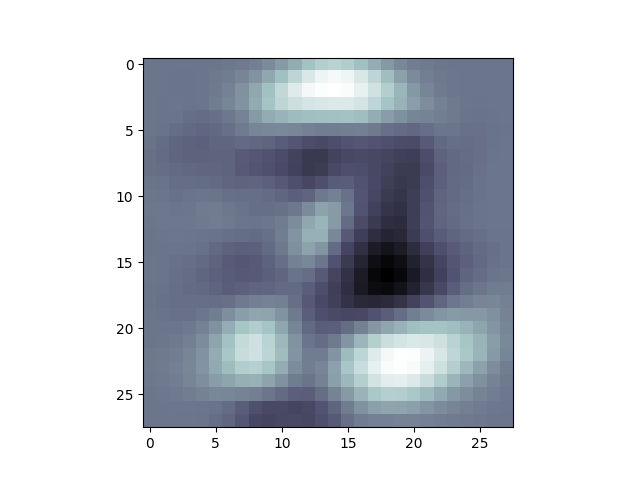
\includegraphics[]{lr2.png}
\end{figure}
\\ \\ \\
logistic\textunderscore regression\textunderscore classification\textunderscore report:
\begin{verbatim}
Classification Report
             precision    recall  f1-score   support

          0       0.98      0.97      0.97       258
          1       0.89      0.89      0.89       258
          2       0.93      0.88      0.90       258
          3       0.97      0.84      0.90       258
          4       0.97      0.87      0.92       258
          5       0.90      0.86      0.88       258
          6       0.92      0.97      0.94       258
          7       0.90      0.96      0.93       258
          8       0.79      0.90      0.84       258
          9       0.79      0.86      0.83       258

avg / total       0.90      0.90      0.90      2580 
\end{verbatim}
logistic\textunderscore regression \textunderscore confusion \textunderscore matrix: \\
 \csvautotabular{logistic_regression_confusion_matrix.csv} \\ \\ \\
logistic\textunderscore regression \textunderscore accuracy: \\
\begin{verbatim}
train_accuracy,test_accuracy
20.9265895953757225,0.8992248062015504
\end{verbatim}

\begin{figure}[h]
\center
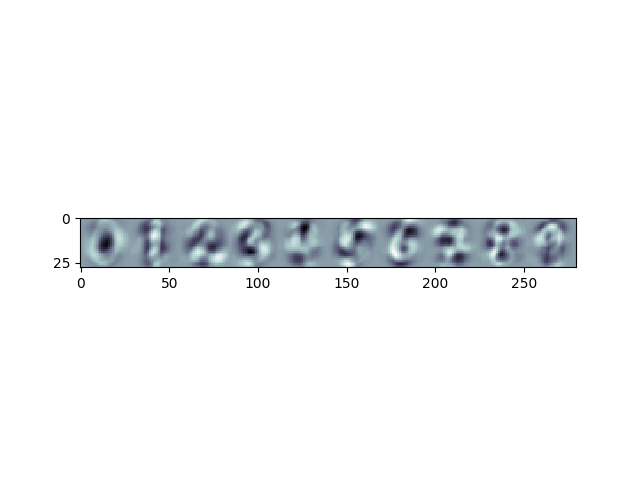
\includegraphics[trim={0 4.5cm 0 5cm},clip]{logistic_regression_parameter_plot_1_128.png}
\end{figure}

logistic\textunderscore regression \textunderscore validation \textunderscore scores: \\
\csvautotabular{logistic_regression_validation_scores.csv} \\ \\ \\

logistic\textunderscore regression \textunderscore best \textunderscore results: \\
\csvautotabular{logistic_regression_best_result.csv} \\ \\ \\

\begin{figure}[h]
\center
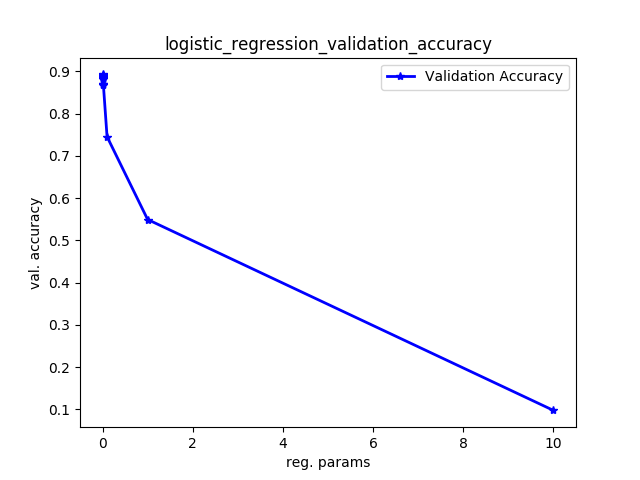
\includegraphics[]{logistic_regression_validation_accuracy.png}
\end{figure}

\subsubsection{Weight Parameter}
The 2 vs 7 parameters weighs heigh when the two is present and seven is not. For instance just above the horizontal top line in seven several people probably makes a curly line for the two instead. Also in the right bottom the two is present but seven is not. \\ \\
It looks like the actual numbers. It makes sense that the algorithms has large weights at the positions of the pixels of the numbers it tries to model. Then the dot product will be large and it will likely be classified as the correct digit.

\subsubsection{Best parameters}
The best regularization parameter is 1e-10. Validation accuracy is 0.893 and test accuracy is 0.893.

\subsection{Theory}

\subsubsection{Question 1}

The running time of logitstic regression is: \\ 
Preprocessing: $\mathcal{O}(n)$ \\
Logcost: $\mathcal{O}(nd)$ (assuming naive matrix multiplication) \\
Gradient: $\mathcal{O}(nd)$ (assuming naive matrix multiplication) \\
\\
The running time of gradient descent is \\
Total: $\mathcal{O}(epochs * logcost) = \mathcal{O}(epochs * n * d)$ \\
The running time of mini gradient descent is \\
Total: $\mathcal{O}(epochs * n/batchsize * batchsize * d) = \mathcal{O}(epochs * n d)$

\subsubsection{Question 2}
The running itme of logistic regression for two classes are: \\
$\mathcal{O}(epochs * n * d)$ \\
Since we just have to do one mini gradient descent.
For K classes we have to do K gradient descents whichs gives a running time of \\
$\mathcal{O}(epochs * n * d * K)$ \\

\subsubsection{Question 3 }
The algorithm only looks at individual pixels so as long as the same permutation is done to all the images there should be no difference.

\section{PART II: Softmax Regression}

\subsection{Code}

\subsubsection{Summary}
We achieved a validation accuracy of 0.903 and test accuracy of 0.776 using regularization parameter of 1e-10. The generalization seems to be very bad for some unknown reason. 

\subsubsection{Results and plots}
softmax\textunderscore classification \textunderscore report
\begin{verbatim}
Classification Report
             precision    recall  f1-score   support

          0       0.94      0.96      0.95       258
          1       0.89      0.81      0.85       258
          2       0.92      0.82      0.87       258
          3       0.85      0.93      0.89       258
          4       0.79      0.91      0.85       258
          5       0.94      0.80      0.87       258
          6       0.92      0.90      0.91       258
          7       0.83      0.95      0.88       258
          8       0.80      0.86      0.83       258
          9       0.85      0.74      0.79       258

avg / total       0.87      0.87      0.87      2580
\end{verbatim}

softmax\textunderscore confusion \textunderscore matrix: \\
 \csvautotabular{softmax_confusion_matrix.csv} \\ \\ \\
softmax\textunderscore accuracy: \\
\begin{verbatim}
train_accuracy,test_accuracy
0.8713872832369942,0.8674418604651163
\end{verbatim}

\begin{figure}[h]
\center
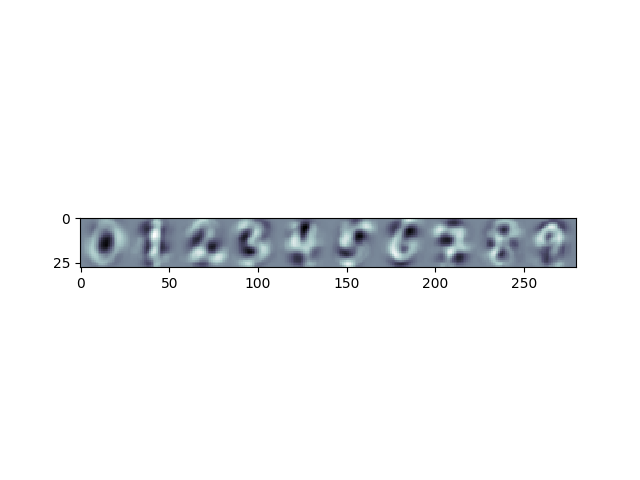
\includegraphics[trim={0 4.5cm 0 5cm},clip]{softmax_parameter_plot_1_128.png}
\end{figure}

softmax\textunderscore validation \textunderscore scores: \\
\csvautotabular{softmax_validation_scores.csv} \\ \\ \\

softmax\textunderscore best \textunderscore results: \\
\csvautotabular{softmax_best_result.csv} \\ \\ \\

`\begin{figure}[h]
\center
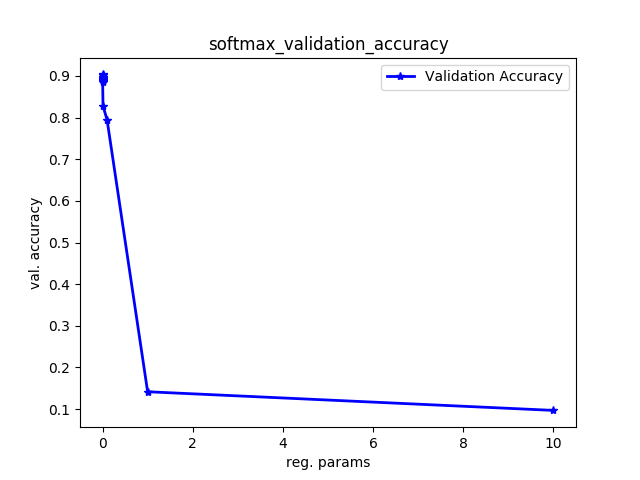
\includegraphics[]{softmax_validation_accuracy.png}
\end{figure}


\subsubsection{Weight parameters}
Looks identical to the parameters for the logistic regression.

\subsubsection{Best Parameters}
Best regularization is 1e-10 which gives an validation accuracy of 0.903 and test accuracy of 0.776.

\subsection{Theory}

\subsubsection{Question 1}

The running time of softmax is: \\ 
Softcost: $\mathcal{O}(ndK)$ (assuming naive matrix multiplication) \\
Gradient: $\mathcal{O}(ndK)$ (assuming naive matrix multiplication) \\
\\
The running time of mini gradient descent is \\
Total: $\mathcal{O}(epochs * n/batchsize * batchsize * d * K) = \mathcal{O}(epochs * ndK)$

Softmax is done by running mini gradient descent one time which makes the above time complexity the time complexity of softmax.

\section{Part III: Softmax vs Logistic Regression}
The logistic regression model turned out to have a better generalization to the test set, but achieved a slightly larger in-sample error. We expect the two methods to be comparable in performance since both have (d + 1) x K parameters. 

\end{document}